\subsection{Submission Confirmation and Complaint Management}
Once a student successfully submits their application form, the system displays a confirmation message and provides options for subsequent necessary actions. This interface ensures the applicants that their data has been securely stored in the database.

\begin{figure}[htbp]
    \centering
    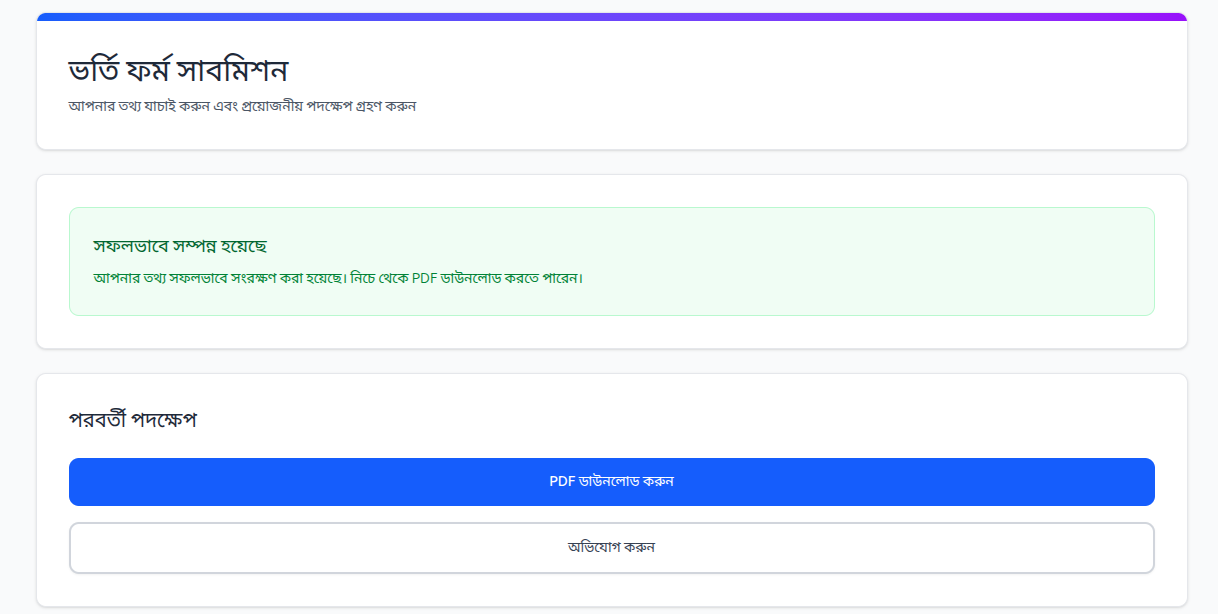
\includegraphics[width=0.85\textwidth]{chapters/chapter4/images/complain.png}
    \caption{Form Submission Confirmation and Complaint Interface}
    \label{fig:submission_status}
\end{figure}

As illustrated in Figure \ref{fig:submission_status}, the submission status page includes several key functional elements:

\begin{itemize}
    \item \textbf{Success Notification:} A green alert box is utilized to inform the student that their information has been successfully saved. This enhances the user experience and maintains system transparency.
    \item \textbf{PDF Generation and Download:} Students can download their completed application form in PDF format for future reference. This is a core component of the system's automated report generation module.
    \item \textbf{Complaint Management:} If a student notices any discrepancy in their data or encounters issues after submission, they can directly file a report through this integrated module.
    \item \textbf{Action Buttons:} The interface features clear and actionable buttons (e.g., "Download PDF" and "Complain"), which guide the user through the next steps without ambiguity.
\end{itemize}

Through this feature, system reliability is increased, and students are provided with immediate feedback and support options.